 \subsection{Floorplan der 2D-DFT-Einheit mit 3 Metalllagen und 350nm Strukturgröße}
 
  In den folgenden Bildern \ref{pic:floorplan1} bis \ref{pic:floorplan4} ist zusehen, wie der Floorplan eine Stromversorgung für die Standardzellen erhält. 
  In Abbildung \ref{pic:floorplan1} ist noch keinerlei Stromversorgung vorhanden. Als erstes wird, wie in Abb. \ref{pic:floorplan2} zu sehen, der äußere Ring gesetzt, welcher alle weiteren
  Verbindungen mit Strom versorgt. Die unterschiedlichen Farben stehen für verschiedene Ebenen des Chips. Bei rot handelt es sich um die zweite, bei grün um 
  die dritte Lage. Besser zu sehen ist die in Abbildung \ref{pic:floorplanVias}. Dort lassen sich auch die zur Durchkontaktierung der einzelnen Lagen genutzten 
  Vias erkennen (rot eingekreist). Desweiteren lassen sich Masse (innerer Ring) und Spannungsversorgung ($V_{dd}$, äußerer Ring) unterscheiden.
  Ersichtlich ist darüber hinaus, dass für die horizontalen und vertikalen Leitungen unterschiedliche Lagen genutzt werden. Auf diese Weise wird vermieden, 
  dass es zu ungewollten Verbindungen von Leitungen kommt.
  In Abbildung \ref{pic:floorplan3} werden, wieder auf Layer zwei, vertikalen Leitungen zur Stromversorgung der Standardzellen hinzugefügt. Auf Bild \ref{pic:floorplan4} werden abschließend auf 
  Layer eins horizontale Verbindungen ergänzt. Auf diese Weise ist die Voraussetzung geschaffen, dass aktive Standardzellen mit Strom versorgt werden können und
  die Netzliste aus Abbildung \ref{pic:Netzliste2D-DFT} auf den Floorplan übertragen werden kann. Das Resultat davon ist in Abbildung \ref{pic:floorplan1Standardzellen}
  zu sehen. 
  
    \begin{figure*}
        \centering
        \begin{subfigure}[b]{0.475\textwidth}
            \centering
            
\includegraphics[width=\textwidth]{img/DFT_FLOORPLAN/CROPPED_IMG/FP_1.png}
            \caption{{\small Leerer Floorplan}}    
            \label{pic:floorplan1}
        \end{subfigure}
        \hfill
        \begin{subfigure}[b]{0.475\textwidth}  
            \centering 
            
\includegraphics[width=\textwidth]{img/DFT_FLOORPLAN/CROPPED_IMG/FP_2.png}
            \caption{{\small Floorplan mit Power-Ring}}    
            \label{pic:floorplan2}
        \end{subfigure}
        \vskip\baselineskip
        \begin{subfigure}[b]{0.475\textwidth}   
            \centering 
            
\includegraphics[width=\textwidth]{img/DFT_FLOORPLAN/CROPPED_IMG/FP_3.png}
            \caption{{\small Floorplan mit vertikaler Stromversorgung auf Metal-Layer 2}}    
            \label{pic:floorplan3}
        \end{subfigure}
        \quad
        \begin{subfigure}[b]{0.475\textwidth}   
            \centering 
            
\includegraphics[width=\textwidth]{img/DFT_FLOORPLAN/CROPPED_IMG/FP_4.png}
            \caption{{\small Floorplan mit zusätzlicher horizontaler Stromversorgung auf Metal-Layer 1}}    
            \label{pic:floorplan4}
        \end{subfigure}
        \caption{Schrittweiser Entwurf der Stromversorgung des Floorplans} 
        \label{fig:floorplanSpannungsversorgung}
    \end{figure*}

    
    \begin{figure}[ht!]
     \centering
     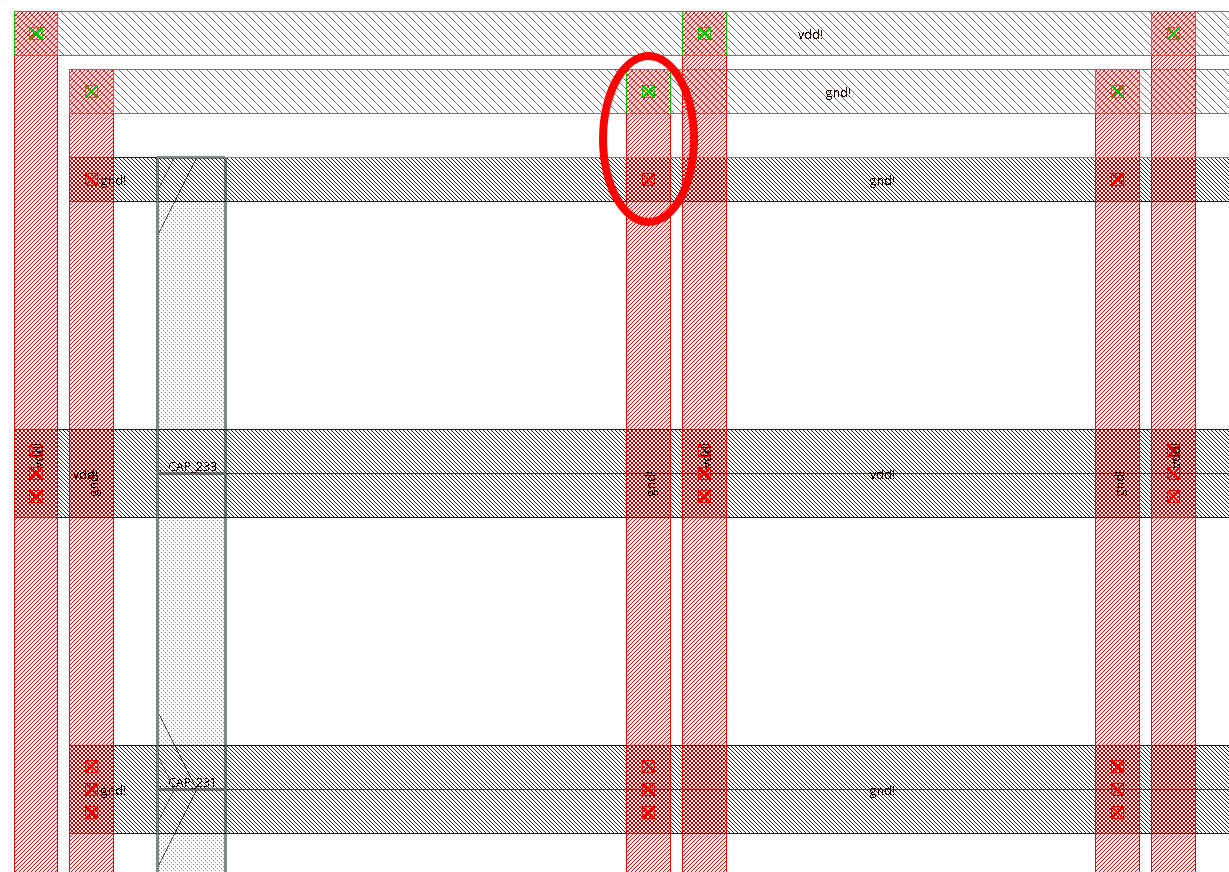
\includegraphics[width=0.88\textwidth]{img/DFT_FLOORPLAN/CROPPED_IMG/Vias.png}
     \caption{Vias für die Durchkontaktierung der Stromversorgung auf den verschiedenen Metalllagen (blau: Layer 1, rot: Layer 2, grün: Layer 3).}
     \label{pic:floorplanVias}
    \end{figure}
    
    
    \begin{figure}[ht!]
     \centering
     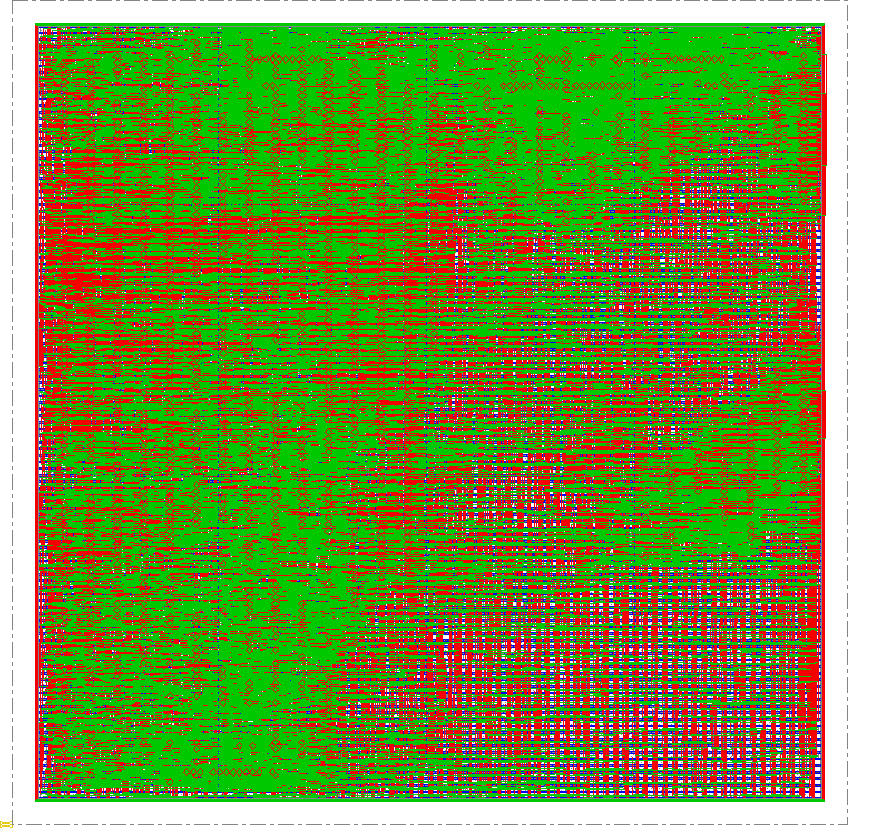
\includegraphics[width=0.88\textwidth]{img/DFT_FLOORPLAN/CROPPED_IMG/FP_5.png}
     \caption{Floorplan mit platzierten Standardzellen der 2D-DFT-Einheit.}
     \label{pic:floorplan1Standardzellen}
    \end{figure}